% Select one class
%\documentclass{pucthesis}		% For DVI
%\documentclass[pdftex]{pucthesis}	% For pdfLaTeX
%\documentclass[spanish]{pucthesis}		% For DVI, in spanish
\documentclass[pdftex,spanish]{pucthesis}	% For pdfLaTeX, in spanish

%%%%%%%%%%%%%%%%%%%%%%%%%%
%      Nota: si usas español, algunos nombres      %
%      debes cambiarlos manualmente en este     %
%        documento. En teoría, nunca deberías       %
%           modificar el archivo pucthesis.cls              %
%%%%%%%%%%%%%%%%%%%%%%%%%%

%%%%%%%%%
%   Packages	 %
%%%%%%%%%

% Floats
\usepackage{graphicx}
\usepackage{float}
\floatstyle{boxed}
\restylefloat{figure}
\IfFileExists{subfigure.sty}{\usepackage{subfigure}}{}  % no está en el TeX Live local; en Overleaf sí
\usepackage{color}

% Math packages
\usepackage{amsmath}
\usepackage{amsfonts}
\usepackage{amssymb}

% Closest font to Times New Roman
\usepackage{times}

% To make pretty tables
\usepackage{booktabs}
\usepackage{multirow}

% To avoid underfull errors in the bibliography
\usepackage{etoolbox}
\apptocmd{\sloppy}{\hbadness 10000\relax}{}{}

% To make cites and references
\usepackage[hidelinks,pdfusetitle,pdfdisplaydoctitle]{hyperref}
\usepackage[notocbib]{apacite} 
\usepackage{doi}
\renewcommand{\doitext}{}

%--------- NEW ENVIRONMENTS --------- You are free to remove or use it
\newtheorem{definition}{\bf Definition}[chapter]
\newtheorem{property}{Property}[chapter]
\newtheorem{claim}{Claim}[chapter]
\newtheorem{lemma}{\bf Lemma}[chapter]
\newtheorem{proposition}{Proposition}[chapter]
\newtheorem{theorem}{\noindent \bf Theorem}[chapter]
\newtheorem{corollary}{\bf Corollary}[chapter]
\newtheorem{pf}{Proof}[chapter]
\newtheorem{example}{\bf Example}[chapter]
\newtheorem{remark}{Remark}[chapter]

% En caso de que el título sea muy largo, se puede ajustar el espacio
% antes y después de este en las dos primeras páginas para que quede centrado.

%\makeatletter
%  \setlength{\beftitle}{105\p@\@plus24\p@}
%  \setlength{\afttitle}{65\p@}
%\makeatother

% Agregados del informe 2 (paquetes y cifras; no cambian la configuración de la plantilla)
\usepackage{tikz}
\usetikzlibrary{positioning,arrows.meta}
% Generado por scripts/cifras.py. No editar a mano.
\newcommand{\AhorroBusesBusqueda}{141}
\newcommand{\AhorroBusesConstruccion}{495}
\newcommand{\ArcosFaseUno}{2.092.978}
\newcommand{\Autonomia}{225}
\newcommand{\Bateria}{350}
\newcommand{\BrechaBusesFaseUno}{8,8}
\newcommand{\BrechaBusesSimultaneidad}{14,0}
\newcommand{\BrechaCostoPiso}{7,5}
\newcommand{\BusesBase}{4.509}
\newcommand{\BusesConDeficit}{3.873}
\newcommand{\BusesConstruccion}{4.014}
\newcommand{\BusesExtraSinRecargas}{1.589}
\newcommand{\BusesModelo}{3.873}
\newcommand{\BusesParejas}{3.989}
\newcommand{\BusesPrototipo}{4.175}
\newcommand{\BusesPrototipoSinMejora}{4.322}
\newcommand{\BusesSinRecargas}{5.150}
\newcommand{\BusesTrios}{3.884}
\newcommand{\BusesUmbralCincuenta}{5.518}
\newcommand{\BusesUmbralTreinta}{4.822}
\newcommand{\BusesUmbralVeinte}{4.516}
\newcommand{\CapacidadECinco}{150}
\newcommand{\CapacidadECuatro}{100}
\newcommand{\CapacidadEDos}{180}
\newcommand{\CapacidadETres}{120}
\newcommand{\CapacidadEUno}{150}
\newcommand{\ConexionesECincoBase}{100}
\newcommand{\ConexionesECincoModelo}{16}
\newcommand{\ConexionesECuatroBase}{69}
\newcommand{\ConexionesECuatroModelo}{16}
\newcommand{\ConexionesEDosBase}{125}
\newcommand{\ConexionesEDosModelo}{14}
\newcommand{\ConexionesETresBase}{53}
\newcommand{\ConexionesETresModelo}{8}
\newcommand{\ConexionesEUnoBase}{74}
\newcommand{\ConexionesEUnoModelo}{12}
\newcommand{\Consumo}{1,4}
\newcommand{\CorridasMuestra}{33.220}
\newcommand{\CorridasRed}{64.502}
\newcommand{\CostoAjustadoBase}{1.694.796}
\newcommand{\CostoAjustadoModelo}{1.483.801}
\newcommand{\CostoBase}{1.601.775}
\newcommand{\CostoBus}{250}
\newcommand{\CostoConEsperaBase}{1.631.153}
\newcommand{\CostoConEsperaModelo}{1.400.339}
\newcommand{\CostoConstruccion}{1.415.349}
\newcommand{\CostoEnergiaBase}{47.769}
\newcommand{\CostoEnergiaModelo}{4.382}
\newcommand{\CostoEsperaBase}{29.378}
\newcommand{\CostoEsperaMinuto}{0,03}
\newcommand{\CostoEsperaModelo}{25.707}
\newcommand{\CostoFlotaBase}{1.127.250}
\newcommand{\CostoFlotaModelo}{968.250}
\newcommand{\CostoKmBase}{422.406}
\newcommand{\CostoKmModelo}{399.329}
\newcommand{\CostoKmUnit}{0,5}
\newcommand{\CostoModelo}{1.374.632}
\newcommand{\CostoParejas}{1.403.068}
\newcommand{\CostoSesion}{5}
\newcommand{\CostoSesionesBase}{4.350}
\newcommand{\CostoSesionesModelo}{2.670}
\newcommand{\CostoSinRecargas}{1.685.098}
\newcommand{\CostoTrios}{1.378.807}
\newcommand{\CostoUmbralCincuenta}{1.986.474}
\newcommand{\CostoUmbralTreinta}{1.718.697}
\newcommand{\CostoUmbralVeinte}{1.604.873}
\newcommand{\CotaSimultaneidad}{3.398}
\newcommand{\DeficitBase}{930.206}
\newcommand{\DeficitModelo}{1.091.690}
\newcommand{\DeltaBuses}{\ensuremath{-}636}
\newcommand{\DeltaBusesConstruccion}{\ensuremath{-}495}
\newcommand{\DeltaBusesParejas}{\ensuremath{-}520}
\newcommand{\DeltaBusesTrios}{\ensuremath{-}625}
\newcommand{\DeltaCosto}{\ensuremath{-}227.143}
\newcommand{\DeltaCostoAjustado}{\ensuremath{-}210.995}
\newcommand{\DeltaCostoEnergia}{\ensuremath{-}43.387}
\newcommand{\DeltaCostoFlota}{\ensuremath{-}159.000}
\newcommand{\DeltaCostoKm}{\ensuremath{-}23.076}
\newcommand{\DeltaCostoSesiones}{\ensuremath{-}1.680}
\newcommand{\DeltaEnergia}{\ensuremath{-}226.097}
\newcommand{\DeltaKmVacio}{\ensuremath{-}46.153}
\newcommand{\DeltaPctBuses}{\ensuremath{-}14,1}
\newcommand{\DeltaPctBusesConstruccion}{\ensuremath{-}11,0}
\newcommand{\DeltaPctBusesParejas}{\ensuremath{-}11,5}
\newcommand{\DeltaPctBusesTrios}{\ensuremath{-}13,9}
\newcommand{\DeltaPctCosto}{\ensuremath{-}14,2}
\newcommand{\DeltaPctCostoAjustado}{\ensuremath{-}12,4}
\newcommand{\DeltaPctCostoConEspera}{\ensuremath{-}14,2}
\newcommand{\DeltaPctCostoConstruccion}{\ensuremath{-}11,6}
\newcommand{\DeltaPctCostoEnergia}{\ensuremath{-}90,8}
\newcommand{\DeltaPctCostoFlota}{\ensuremath{-}14,1}
\newcommand{\DeltaPctCostoKm}{\ensuremath{-}5,5}
\newcommand{\DeltaPctCostoParejas}{\ensuremath{-}12,4}
\newcommand{\DeltaPctCostoSesiones}{\ensuremath{-}38,6}
\newcommand{\DeltaPctCostoTrios}{\ensuremath{-}13,9}
\newcommand{\DeltaPctEnergia}{\ensuremath{-}89,5}
\newcommand{\DeltaPctKmVacio}{\ensuremath{-}32,9}
\newcommand{\DeltaPctSesiones}{\ensuremath{-}38,6}
\newcommand{\DeltaPpVacio}{\ensuremath{-}4,8}
\newcommand{\DeltaSesiones}{\ensuremath{-}336}
\newcommand{\EnergiaBase}{252.529}
\newcommand{\EnergiaBloque}{15}
\newcommand{\EnergiaModelo}{26.432}
\newcommand{\FlotaFaseUno}{3.561}
\newcommand{\HoraCotaSimultaneidad}{18:30}
\newcommand{\HorasBusMasVacio}{1,8}
\newcommand{\HorasCargaParalelo}{8,7}
\newcommand{\KmBase}{844.811}
\newcommand{\KmModelo}{798.659}
\newcommand{\KmServicio}{704.414}
\newcommand{\KmVacioBase}{140.397}
\newcommand{\KmVacioModelo}{94.244}
\newcommand{\MedianaAhorroCientoVeinte}{24.927}
\newcommand{\MedianaAhorroDosCuarenta}{30.295}
\newcommand{\MedianaAhorroQuince}{8.997}
\newcommand{\MedianaAhorroSesenta}{17.320}
\newcommand{\MedianaAhorroTreinta}{14.582}
\newcommand{\MedianaBusesEvitadosCientoVeinte}{91}
\newcommand{\MedianaBusesEvitadosDosCuarenta}{107}
\newcommand{\MedianaBusesEvitadosQuince}{35}
\newcommand{\MedianaBusesEvitadosSesenta}{63}
\newcommand{\MedianaBusesEvitadosTreinta}{56}
\newcommand{\MinutosEsperaBase}{979.271}
\newcommand{\MinutosEsperaModelo}{856.896}
\newcommand{\MinutosRefinado}{28,6}
\newcommand{\ModelosDescartados}{184}
\newcommand{\ModelosLocales}{60.440}
\newcommand{\NodosFaseUno}{63.298}
\newcommand{\PctAhorroConstruccion}{77,8}
\newcommand{\PctCorridasMuestra}{51,5}
\newcommand{\PctEnergiaBase}{3,0}
\newcommand{\PctEnergiaModelo}{0,3}
\newcommand{\PctEnergiaPuntaBase}{64,8}
\newcommand{\PctEnergiaPuntaModelo}{29,3}
\newcommand{\PctFlotaBase}{70,4}
\newcommand{\PctFlotaModelo}{70,4}
\newcommand{\PctKmBase}{26,4}
\newcommand{\PctKmModelo}{29,0}
\newcommand{\PctRutasMuestra}{50,8}
\newcommand{\PctSesionesBase}{0,3}
\newcommand{\PctSesionesModelo}{0,2}
\newcommand{\PctVacioBase}{16,6}
\newcommand{\PctVacioModelo}{11,8}
\newcommand{\PctVacioUmbralCincuenta}{23,0}
\newcommand{\PctVacioUmbralTreinta}{18,0}
\newcommand{\PctVacioUmbralVeinte}{16,7}
\newcommand{\PisoFaseUno}{1.278.245}
\newcommand{\PlazasECincoBase}{100}
\newcommand{\PlazasECincoModelo}{150}
\newcommand{\PlazasECuatroBase}{69}
\newcommand{\PlazasECuatroModelo}{100}
\newcommand{\PlazasEDosBase}{125}
\newcommand{\PlazasEDosModelo}{180}
\newcommand{\PlazasETresBase}{53}
\newcommand{\PlazasETresModelo}{120}
\newcommand{\PlazasEUnoBase}{74}
\newcommand{\PlazasEUnoModelo}{150}
\newcommand{\PlazasTotales}{700}
\newcommand{\Potencia}{180}
\newcommand{\PrecioMedioKwhBase}{0,189}
\newcommand{\PrecioMedioKwhModelo}{0,166}
\newcommand{\Reserva}{35}
\newcommand{\RondasCarga}{6}
\newcommand{\RutasMuestra}{212}
\newcommand{\RutasRed}{417}
\newcommand{\SesionesBase}{870}
\newcommand{\SesionesModelo}{534}
\newcommand{\TarifaNocturna}{0,10}
\newcommand{\TarifaPunta}{0,22}
\newcommand{\VelocidadVacio}{18}


\begin{document}

\mdate{Octubre 2026}
\version{2}

\title[PLANIFICACIÓN DE LA OPERACIÓN DE BUSES ELÉCTRICOS EN LA REGIÓN METROPOLITANA\\ GRUPO 29]
   {\bf PLANIFICACIÓN DE LA OPERACIÓN DE BUSES ELÉCTRICOS EN LA REGIÓN METROPOLITANA\\ GRUPO 29}
\author[Integrantes:]{Integrantes:\\
\textnormal{\small{
Gonzalo Anguita\\
Diego Barrios\\
Gustavo Cueto\\
Nicolás Farías\\
Fernando González\\
Ricardo Palma\\
Cristóbal Rehbein}
}
}

\address{Escuela de Ingenier\'ia\\
                   Pontificia Universidad Cat\'olica de Chile\\
                   Vicu\~na Mackenna 4860\\
                  Santiago, Chile\\
                  {\it Tel.\/} : 56 (2) 354-2000}

\advisor                    {\textbf{Profesor Guía:} Agustín Chiu}
\ogrsmember                 {\textbf{Ayudante Tutor:} Max Burr}
\date                       {Octubre 2026}
\copyrightname              {Grupo 29}
\copyrightyear              {2026}

\NoChapterPageNumber
\pagenumbering{roman}
\maketitle

\pdfbookmark{\contentsname}{toc}
\tableofcontents
\phantomsection \label{listoffigures}
\listoffigures
\phantomsection \label{listoftables}
\listoftables
\cleardoublepage

\phantomsection \label{resumen}
\chapter*{RESUMEN}
% Se redacta según ESQUEMA.md. Archivo: resumen

\cleardoublepage

\pagenumbering{arabic}

\chapter[INTRODUCCIÓN]{Introducción} \label{ch:introduccion}
% Se redacta según ESQUEMA.md. Archivo: cap01_introduccion


\chapter[DESCRIPCIÓN DETALLADA DEL PROBLEMA Y DATOS]{Descripción detallada del problema y datos} \label{ch:problema}
% Se redacta según ESQUEMA.md. Archivo: cap02_problema_datos


\chapter[EVOLUCIÓN Y DISCUSIÓN METODOLÓGICA]{Evolución y discusión metodológica} \label{ch:evolucion}
% Se redacta según ESQUEMA.md. Archivo: cap03_evolucion
\nocite{*}


\chapter[CASO BASE]{Caso base} \label{ch:caso-base}
% Capítulo 4. Caso base. Spec: ESQUEMA.md §4, capítulo 4.

El caso base es la línea de comparación de los indicadores del capítulo~\ref{ch:resultados}: una forma intuitiva de programar la flota, sin optimización, que incluye la recarga porque es una parte esencial del problema, como observó el equipo docente en la presentación de la Entrega~2.

\section{Política miope por ruta con recarga}
\label{sec:politica-miope}

La política decide corrida por corrida, sin mirar las que vienen después; por eso se le llama miope:

\begin{enumerate}
\item Las corridas se recorren en el orden de su hora de salida.
\item Cada ruta tiene sus propios buses: un bus nunca atiende corridas de dos rutas, aunque ambas sean del mismo sector.
\item Cada corrida se asigna al bus de su ruta que lleva más tiempo libre y alcanza a llegar a tiempo a su inicio.
\item Si la batería no alcanza para la corrida más el regreso a un terminal con la reserva de \Reserva~kWh, el bus va antes al electroterminal más cercano con cupo y carga hasta el 100\,\%, a la tarifa de esa hora; si ahí no alcanza a cargar a tiempo, prueba con el siguiente.
\item Si ningún bus de la ruta puede tomar la corrida, se agrega uno nuevo, con la batería llena, desde el terminal de espera más cercano.
\item Después de su última corrida, cada bus vuelve al terminal de espera más cercano.
\end{enumerate}

\section{Por qué es una línea base defendible}
\label{sec:caso-base-defendible}

La política reproduce cómo se programaría la flota sin investigación operativa: buses asignados a una ruta que recargan cuando hace falta, como un bus diésel que carga combustible cuando se le acaba. No resuelve ningún modelo, así que toda diferencia con el modelo proviene de coordinar mejor las decisiones. La comparación se hace en el mismo terreno: las mismas \RutasMuestra{} rutas y \CorridasMuestra{} corridas laborales del modelo, es decir, la misma instancia reducida del capítulo~\ref{ch:problema}, con el mismo horizonte, las mismas constantes y los mismos electroterminales. Su plan se revisó con el mismo auditor que revisa las soluciones del modelo (cobertura exacta, continuidad, energía, reserva y capacidades compartidas), que lo aprobó y reprodujo sin diferencias sus buses, kilómetros, energía, sesiones y costo. La implementación tiene seis pruebas automáticas propias. Su limitación al comparar es que, como siempre carga hasta el 100\,\%, termina el día con más energía en las baterías que el modelo; por eso se compara también un costo ajustado por la energía final (sección~\ref{sec:energia}).

Este caso base reemplaza al de la presentación de la Entrega~2, que no recargaba: cortaba las cadenas de corridas del prototipo anterior (capítulo~\ref{ch:evolucion}) en jornadas dentro de la autonomía de \Autonomia~km y necesitaba \BusesSinRecargas{} buses y USD~\CostoSinRecargas{} al día. Se reemplazó porque una línea base sin recarga deja fuera una parte esencial del problema y exagera la ganancia de cualquier modelo que sí recargue. Lo que mostraba sigue siendo útil: sin recarga, \BusesExtraSinRecargas{} cadenas necesitan un segundo bus solo porque la batería no alcanza. Cómo se cubre el día siguiente se discute en el capítulo~\ref{ch:supuestos}.

\section{Resultado y sensibilidad al umbral de carga}
\label{sec:resultado-caso-base}

La Tabla~\ref{tab:caso-base} resume el plan. La flota explica el \PctFlotaBase\,\% del costo y los kilómetros, el \PctKmBase\,\%; la electricidad y las sesiones pesan poco en el costo, aunque determinan cuántos buses hacen falta. Como cada ruta reposiciona sus propios buses, el \PctVacioBase\,\% de los kilómetros se recorre sin pasajeros.

\begin{table}[htbp]
\centering
\caption{Plan del caso base miope (\RutasMuestra{} rutas, día laboral, umbral de carga de 0\,\%).}
\label{tab:caso-base}
\begin{tabular}{lrr}
\toprule
Indicador & Valor & \% del costo total \\
\midrule
Buses utilizados & \BusesBase & --- \\
Costo total (USD/día) & \CostoBase & 100 \\
\quad Flota & \CostoFlotaBase & \PctFlotaBase \\
\quad Kilómetros & \CostoKmBase & \PctKmBase \\
\quad Electricidad & \CostoEnergiaBase & \PctEnergiaBase \\
\quad Sesiones de carga & \CostoSesionesBase & \PctSesionesBase \\
Kilómetros en vacío & \PctVacioBase\,\% del total & --- \\
\bottomrule
\end{tabular}
\end{table}

La política admite un umbral: con un umbral de 30\,\%, por ejemplo, el bus va a cargar apenas su batería baja del 30\,\%, aunque todavía le alcance para la corrida siguiente. Subir el umbral solo empeora el caso base, porque multiplica las visitas a los electroterminales: con umbrales de 20, 30 y 50\,\% necesita \BusesUmbralVeinte, \BusesUmbralTreinta{} y \BusesUmbralCincuenta{} buses y cuesta USD~\CostoUmbralVeinte, \CostoUmbralTreinta{} y \CostoUmbralCincuenta{} al día. Para no inflar la ganancia del modelo se usa el umbral de 0\,\%, el más favorable.


\chapter[METODOLOGÍA HÍBRIDA PROPUESTA]{Metodología híbrida propuesta} \label{ch:metodologia}
% Se redacta según ESQUEMA.md. Archivo: cap05_metodologia


\chapter[IMPLEMENTACIÓN COMPUTACIONAL Y TRAZABILIDAD]{Implementación computacional y trazabilidad} \label{ch:implementacion}
% Capítulo 6. Implementación computacional y trazabilidad. Spec: ESQUEMA.md §4, capítulo 6.

El método del capítulo~\ref{ch:metodologia} está implementado en Python, en la carpeta \texttt{metodo\_hibrido} del repositorio del proyecto (\url{https://github.com/nfariasl/capstone-grupo29}). Aquí se describe su organización, sus herramientas, su verificación y cómo se reproduce la solución del capítulo~\ref{ch:resultados}.

\section{Módulos y flujo de ejecución}
\label{sec:modulos}

La Figura~\ref{fig:flujo} muestra el orden en que trabajan los módulos. La instancia (corridas, distancias viales y parámetros del escenario) se lee una vez. La construcción cronológica arma un plan inicial factible; el archivo que la implementa se llama \texttt{caso\_base.py} por razones históricas, pero no es el caso base del capítulo~\ref{ch:caso-base}. Después, las búsquedas por parejas y por tríos proponen cambios entre jornadas, y para cada propuesta un modelo de programación entera mixta (MILP) local decide las recargas y los terminales de esas jornadas. Ningún cambio se acepta sin pasar por el auditor. Al final se exportan el plan de cada bus, sus actividades, sus recargas y un resumen de indicadores.

\begin{figure}[htbp]
\centering
\begin{tikzpicture}[node distance=9mm and 5mm, caja/.style={draw, rounded corners, align=center,
  font=\footnotesize, minimum height=11mm, text width=26mm}, flecha/.style={-Stealth}]
\node[caja] (inst) {Instancia\\\scriptsize\texttt{instancia\_212/}};
\node[caja, right=of inst] (cons) {Construcción\\cronológica\\\scriptsize\texttt{caso\_base.py}};
\node[caja, right=of cons] (par) {Parejas\\\scriptsize\texttt{intercambios.py}};
\node[caja, right=of par] (tri) {Tríos\\\scriptsize\texttt{trios.py}};
\node[caja, below=of tri] (milp) {MILP local\\\scriptsize\texttt{conjunta.py}\\\texttt{recarga.py}};
\node[caja, below=of par] (aud) {Auditoría\\\scriptsize\texttt{verificar.py}\\\scriptsize acepta si baja el costo};
\node[caja, below=of cons] (exp) {Exportación\\\scriptsize\texttt{ejecutar.py}\\\texttt{buscar\_mejor.py}};
\draw[flecha] (inst) -- (cons);
\draw[flecha] (cons) -- (par);
\draw[flecha] (par) -- (tri);
\draw[flecha] (tri) -- (milp);
\draw[flecha] (milp) -- (aud);
\draw[flecha] (aud) -- (exp);
\end{tikzpicture}
\caption{Módulos del método híbrido y orden en que se ejecutan. Las búsquedas por parejas y por tríos llaman al MILP local para cada cambio que proponen.}
\label{fig:flujo}
\end{figure}

\section{Herramientas}
\label{sec:herramientas}

El código usa Python~3.12 y NumPy. Los modelos locales se resuelven con Gurobi~12 a través de su interfaz \texttt{gurobipy}, con la licencia restringida que se instala con el paquete, que admite hasta dos mil variables y dos mil restricciones por modelo, con un límite de dos segundos cada uno. En la búsqueda que produjo la solución informada se resolvieron \ModelosLocales{} modelos locales y se descartaron \ModelosDescartados{} que superaban ese tamaño.

\section{Verificación}
\label{sec:verificacion}

El auditor (\texttt{verificar.py}) es independiente del constructor y de las búsquedas: reconstruye cada plan desde sus actividades y comprueba que cada corrida se cubra exactamente una vez, con su horario y sus paradas; que cada bus pueda llegar a tiempo de una actividad a la siguiente; que una jornada no cruce sectores; que la energía nunca baje de la reserva, y que las plazas y conexiones de cada electroterminal nunca se excedan. Cada etapa trabaja sobre una copia del plan y solo reemplaza a la anterior si el auditor la aprueba y su costo es estrictamente menor. El código tiene 22 pruebas automáticas (14 de la construcción y 8 de las búsquedas), todas aprobadas con la versión usada aquí.

\section{Trazabilidad y reproducción}
\label{sec:reproduccion}

Cada corrida guarda sus parámetros, las versiones de Python, NumPy y Gurobi, y la huella SHA-256 de cada archivo de entrada y de código (\texttt{ejecucion.json}); la solución final guarda además la huella de cada archivo exportado (\texttt{verificacion\_final.json}). El código del repositorio coincide con esas huellas, salvo \texttt{buscar\_mejor.py}, al que después de obtener la solución se le agregó la opción de elegir la instancia. Las cifras de este informe las genera un script desde esos archivos, así que cada número es rastreable. La solución informada se obtuvo en dos pasos, una búsqueda de 600 segundos por etapa desde la construcción y un refinamiento de 240 segundos desde ese resultado (\MinutosRefinado{} minutos en total); como el presupuesto es de reloj, repetirlos entrega una solución similar, pero no idéntica (sección~\ref{sec:variabilidad}):

\begin{small}
\begin{verbatim}
python metodo_hibrido/buscar_mejor.py --salida mejor_600 \
    --presupuesto 600 --vecinos 8 --alternativas 3 --rondas 30 \
    --licencia-restringida
python metodo_hibrido/buscar_mejor.py --salida refinamiento \
    --desde mejor_600/04_final/planes.json \
    --presupuesto 240 --vecinos 12 --alternativas 5 --rondas 30 \
    --licencia-restringida
\end{verbatim}
\end{small}


\chapter[RESULTADOS Y ANÁLISIS DE KPIS]{Resultados y análisis de KPIs} \label{ch:resultados}
% Capítulo 7. Resultados y análisis de KPIs. Spec: ESQUEMA.md §4, capítulo 7.

Este capítulo compara el plan del modelo híbrido (la mejor solución encontrada, descrita en el capítulo~\ref{ch:implementacion}) con el caso base del capítulo~\ref{ch:caso-base}, sobre las mismas \RutasMuestra{} rutas y \CorridasMuestra{} corridas laborales. Todas las tablas muestran el cambio absoluto ($\Delta$) y porcentual ($\Delta\%$) respecto del caso base.

\section{Indicadores principales}
\label{sec:kpis-resultados}

El modelo cubre las mismas corridas con \BusesModelo{} buses, \DeltaBuses{} respecto del caso base (\DeltaPctBuses\,\%), y con un costo de USD~\CostoModelo{} al día, \DeltaPctCosto\,\% menos (Tabla~\ref{tab:kpis}). Los kilómetros en vacío bajan de \PctVacioBase\,\% a \PctVacioModelo\,\% del total, porque un bus del modelo puede tomar corridas de distintas rutas de su sector y encadenar la que empieza más cerca. La energía comprada cae casi a una décima, pero esa cifra no se puede leer sola: el caso base carga siempre hasta el 100\,\% y termina el día con mucha más energía en las baterías (sección~\ref{sec:energia}).

\begin{table}[htbp]
\centering
\caption{Indicadores del caso base y del modelo híbrido (\RutasMuestra{} rutas, día laboral).}
\label{tab:kpis}
\begin{tabular}{lrrrr}
\toprule
Indicador & Caso base & Modelo & $\Delta$ & $\Delta\%$ \\
\midrule
Buses utilizados & \BusesBase & \BusesModelo & \DeltaBuses & \DeltaPctBuses \\
Costo total (USD/día) & \CostoBase & \CostoModelo & \DeltaCosto & \DeltaPctCosto \\
Km en vacío (\% de los km) & \PctVacioBase & \PctVacioModelo & \DeltaPpVacio{} pp & --- \\
Energía comprada (kWh) & \EnergiaBase & \EnergiaModelo & \DeltaEnergia & \DeltaPctEnergia \\
Sesiones de carga & \SesionesBase & \SesionesModelo & \DeltaSesiones & \DeltaPctSesiones \\
\bottomrule
\end{tabular}
\end{table}

\section{Composición del costo}
\label{sec:composicion-costo}

La flota pesa lo mismo en ambos planes, \PctFlotaBase\,\% y \PctFlotaModelo\,\% del costo (Tabla~\ref{tab:costos}), y es la palanca principal: de los USD~\DeltaCosto{} de diferencia diaria, USD~\DeltaCostoFlota{} corresponden a los buses que el modelo deja de usar. Los kilómetros aportan USD~\DeltaCostoKm, por el menor recorrido en vacío. La electricidad y las sesiones pesan poco en el costo (\PctEnergiaModelo\,\% y \PctSesionesModelo\,\% en el modelo), pero cuándo y dónde se carga decide cuántos buses hacen falta: un bus que alcanza a cargar entre dos corridas no necesita un reemplazo.

\begin{table}[htbp]
\centering
\caption{Composición del costo diario (USD/día y porcentaje del costo total de cada plan).}
\label{tab:costos}
\small
\begin{tabular}{lrrrrrr}
\toprule
 & \multicolumn{2}{c}{Caso base} & \multicolumn{2}{c}{Modelo} & & \\
\cmidrule(lr){2-3}\cmidrule(lr){4-5}
Componente & USD & \% & USD & \% & $\Delta$ & $\Delta\%$ \\
\midrule
Flota & \CostoFlotaBase & \PctFlotaBase & \CostoFlotaModelo & \PctFlotaModelo & \DeltaCostoFlota & \DeltaPctCostoFlota \\
Kilómetros & \CostoKmBase & \PctKmBase & \CostoKmModelo & \PctKmModelo & \DeltaCostoKm & \DeltaPctCostoKm \\
Electricidad & \CostoEnergiaBase & \PctEnergiaBase & \CostoEnergiaModelo & \PctEnergiaModelo & \DeltaCostoEnergia & \DeltaPctCostoEnergia \\
Sesiones & \CostoSesionesBase & \PctSesionesBase & \CostoSesionesModelo & \PctSesionesModelo & \DeltaCostoSesiones & \DeltaPctCostoSesiones \\
\midrule
Total & \CostoBase & 100 & \CostoModelo & 100 & \DeltaCosto & \DeltaPctCosto \\
\bottomrule
\end{tabular}
\end{table}

\section{De dónde sale la diferencia}
\label{sec:etapas}

Para saber si la diferencia se debe a un caso base débil o al modelo, la Tabla~\ref{tab:etapas} sigue la solución etapa por etapa. La construcción cronológica (capítulo~\ref{ch:metodologia}), sin ninguna búsqueda local, ya ahorra \AhorroBusesConstruccion{} buses, el \PctAhorroConstruccion\,\% de la reducción total. Respecto del caso base, que también recarga, la construcción cambia tres cosas: los buses se comparten entre las rutas de un mismo sector, cada bus carga solo la energía que necesita en vez de llenar la batería, y cada corrida se asigna al bus disponible con el traslado en vacío más corto. Son decisiones de coordinación del modelo, no un efecto de que el caso base no cargue. La búsqueda local por parejas y tríos, con su refinamiento, aporta los \AhorroBusesBusqueda{} buses restantes. Como las etapas se aplicaron en secuencia, la tabla no aísla el efecto de cada regla por separado.

\begin{table}[htbp]
\centering
\caption{Buses y costo por etapa del método, comparados con el caso base.}
\label{tab:etapas}
\begin{tabular}{lrrrr}
\toprule
Etapa & Buses & Costo (USD/día) & $\Delta$ buses & $\Delta\%$ costo \\
\midrule
Caso base miope & \BusesBase & \CostoBase & --- & --- \\
Construcción cronológica & \BusesConstruccion & \CostoConstruccion & \DeltaBusesConstruccion & \DeltaPctCostoConstruccion \\
\quad + parejas & \BusesParejas & \CostoParejas & \DeltaBusesParejas & \DeltaPctCostoParejas \\
\quad + tríos & \BusesTrios & \CostoTrios & \DeltaBusesTrios & \DeltaPctCostoTrios \\
\quad + refinamiento (modelo) & \BusesModelo & \CostoModelo & \DeltaBuses & \DeltaPctCosto \\
\bottomrule
\end{tabular}
\end{table}

\section{Energía: cuándo y cuánto se carga}
\label{sec:energia}

La Figura~\ref{fig:energia} muestra la energía cargada según la hora del día, coloreada por la tarifa de esa hora. El caso base carga el \PctEnergiaPuntaBase\,\% de su energía en las horas de tarifa más alta (USD~\TarifaPunta{} por kWh), sobre todo al atardecer, cuando las baterías de los buses que partieron en la mañana se agotan. El modelo reparte la carga a lo largo del día y carga parte en la madrugada: solo el \PctEnergiaPuntaModelo\,\% de su energía se paga a la tarifa más alta, y el precio medio que paga baja de USD~\PrecioMedioKwhBase{} a \PrecioMedioKwhModelo{} por kWh.

\begin{figure}[htbp]
\centering
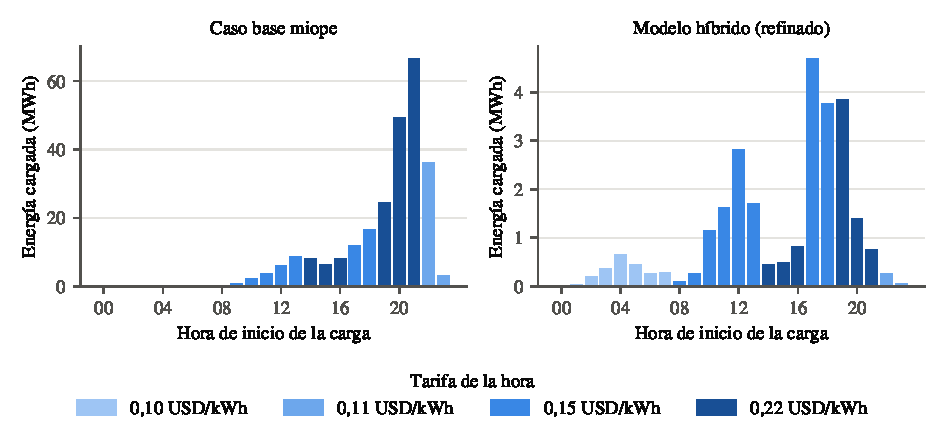
\includegraphics[width=\textwidth]{figures/energia_por_hora.pdf}
\caption{Energía cargada por hora de inicio de la carga, según la tarifa de esa hora. Cada panel tiene su propia escala: el caso base carga cerca de diez veces más energía que el modelo.}
\label{fig:energia}
\end{figure}

La energía comprada no es comparable directamente. Ambos planes parten con las baterías llenas y ninguno paga esa carga inicial, pero terminan con distinta energía: para volver a dejar llenos todos los buses, al caso base le faltan \DeficitBase~kWh y al modelo, \DeficitModelo~kWh. Si esa diferencia se valoriza a la tarifa nocturna de USD~\TarifaNocturna{} por kWh, el costo ajustado es de USD~\CostoAjustadoBase{} para el caso base y USD~\CostoAjustadoModelo{} para el modelo. La ventaja del modelo se reduce de \DeltaPctCosto\,\% a \DeltaPctCostoAjustado\,\%, pero se mantiene. Si esa energía alcanza a reponerse durante la noche es otra pregunta, que se analiza en el capítulo~\ref{ch:supuestos}.

\section{Uso de los electroterminales}
\label{sec:uso-electroterminales}

En el modelo, las plazas de los cinco electroterminales llegan a su capacidad, mientras que las conexiones de carga en uso simultáneo nunca pasan de unas pocas decenas (Tabla~\ref{tab:electroterminales}). El recurso que limita no son los cargadores, sino el espacio físico: los buses ocupan plazas mientras esperan su próxima corrida o al terminar su jornada. En el caso base, la ocupación máxima coincide con las conexiones en uso, porque sus buses solo entran al electroterminal para cargar. Para la entrega final, esto sugiere estudiar más plazas de estacionamiento o un mejor uso de los terminales de espera antes que más cargadores.

\begin{table}[htbp]
\centering
\caption{Ocupación máxima de plazas y conexiones de carga por electroterminal (cada uno tiene tantas conexiones como plazas).}
\label{tab:electroterminales}
\begin{tabular}{lrrrrr}
\toprule
 & & \multicolumn{2}{c}{Plazas ocupadas} & \multicolumn{2}{c}{Conexiones en uso} \\
\cmidrule(lr){3-4}\cmidrule(lr){5-6}
Electroterminal & Plazas & Caso base & Modelo & Caso base & Modelo \\
\midrule
E1 & \CapacidadEUno & \PlazasEUnoBase & \PlazasEUnoModelo & \ConexionesEUnoBase & \ConexionesEUnoModelo \\
E2 & \CapacidadEDos & \PlazasEDosBase & \PlazasEDosModelo & \ConexionesEDosBase & \ConexionesEDosModelo \\
E3 & \CapacidadETres & \PlazasETresBase & \PlazasETresModelo & \ConexionesETresBase & \ConexionesETresModelo \\
E4 & \CapacidadECuatro & \PlazasECuatroBase & \PlazasECuatroModelo & \ConexionesECuatroBase & \ConexionesECuatroModelo \\
E5 & \CapacidadECinco & \PlazasECincoBase & \PlazasECincoModelo & \ConexionesECincoBase & \ConexionesECincoModelo \\
\bottomrule
\end{tabular}
\end{table}

\section{Variabilidad de la búsqueda}
\label{sec:variabilidad}

La búsqueda local se detiene por tiempo de reloj, así que su resultado depende del presupuesto y del equipo. Para medir esa variabilidad se repitió la búsqueda desde la construcción con presupuestos de 15 a 240 segundos por etapa, tres veces cada uno, en un mismo equipo (Anexo~\ref{an:barrido}). La mediana del ahorro sobre la construcción sube de USD~\MedianaAhorroQuince{} al día (\MedianaBusesEvitadosQuince{} buses) con 15 segundos a USD~\MedianaAhorroDosCuarenta{} (\MedianaBusesEvitadosDosCuarenta{} buses) con 240 segundos, sin estabilizarse (Figura~\ref{fig:barrido}). La dispersión entre repeticiones crece con el presupuesto, porque cada repetición alcanza a explorar vecindarios distintos. La mejor solución, obtenida con búsquedas de 600 y 240 segundos por etapa, sigue esa tendencia; más tiempo de búsqueda probablemente reduciría aún más la flota.

\begin{figure}[htbp]
\centering
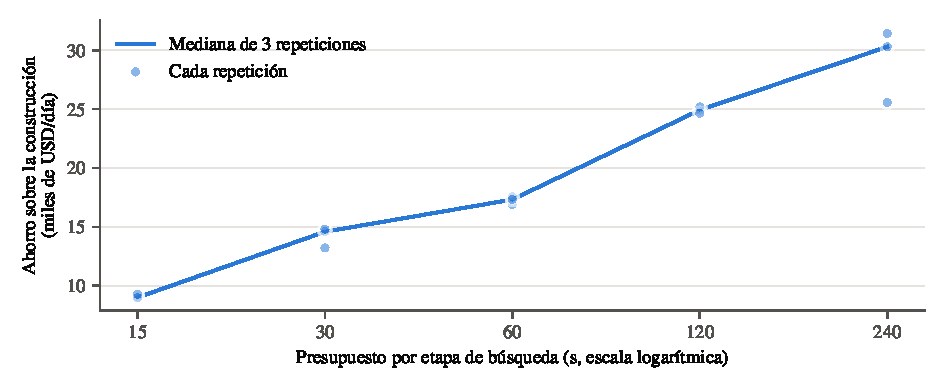
\includegraphics[width=\textwidth]{figures/barrido.pdf}
\caption{Ahorro de la búsqueda local sobre la construcción según el presupuesto por etapa (tres repeticiones por presupuesto, en un mismo equipo).}
\label{fig:barrido}
\end{figure}

\section{Cotas inferiores y brecha}
\label{sec:cotas}

El método no garantiza el óptimo, pero dos cotas inferiores acotan cuánto podría mejorar. La primera es la simultaneidad: a las \HoraCotaSimultaneidad{} hay \CotaSimultaneidad{} corridas en curso a la vez y cada una necesita un bus distinto; el modelo usa \BrechaBusesSimultaneidad\,\% más buses. La segunda es el flujo relajado de la fase~1 del prototipo (capítulo~\ref{ch:evolucion}), que usa los mismos sectores, ignora la batería y se resolvió a optimalidad: \FlotaFaseUno{} buses y USD~\PisoFaseUno{} al día en flota y kilómetros. Como relaja la batería, ningún plan factible con esos sectores puede costar menos. El modelo queda \BrechaCostoPiso\,\% sobre ese piso en costo y \BrechaBusesFaseUno\,\% en buses, de modo que, dentro de la sectorización, su distancia al óptimo es a lo más de \BrechaCostoPiso\,\%. Una cota no necesita ser factible para servir: basta con que ninguna solución factible pueda estar por debajo de ella.

\section{Validez de los indicadores}
\label{sec:validez-kpis}

Los buses utilizados y el costo total distinguen claramente entre el caso base y el modelo y son los que deben guiar la decisión. Los kilómetros en vacío explican parte del costo de kilómetros y muestran el efecto de compartir buses entre rutas. El uso de los electroterminales revela qué recurso limita (las plazas y no los cargadores), así que sirve para decisiones de infraestructura. Los kilómetros de servicio, en cambio, son idénticos en ambos planes (\KmServicio~km), porque dependen solo de las corridas: son un dato del problema y no un indicador. La energía comprada solo es comparable con el ajuste por la energía final, por lo que queda como indicador de apoyo, igual que el tiempo de cómputo.

\section{Limitaciones y mejoras posibles}
\label{sec:limitaciones-resultados}

Los resultados valen para un día laboral aislado, que parte con las baterías llenas y no exige reponerlas al final; esa es la principal limitación y se discute en el capítulo~\ref{ch:supuestos}. La búsqueda terminó por presupuesto y no explora intercambios entre sectores, que hoy están fijos. Tampoco se cobran las esperas, aunque con el costo de espera del enunciado la ventaja del modelo se mantiene en \DeltaPctCostoConEspera\,\% (capítulo~\ref{ch:supuestos}). Las mejoras más directas para la entrega final son dar más presupuesto a la búsqueda o mejorar la construcción, que explica la mayor parte del ahorro; permitir jornadas que crucen sectores, y exigir un estado de carga al final del día.


\chapter[SUPUESTOS, RIESGOS Y PLAN DE SENSIBILIDAD]{Supuestos, riesgos y plan de sensibilidad} \label{ch:supuestos}
% Se redacta según ESQUEMA.md. Archivo: cap08_supuestos


\chapter[CONCLUSIONES]{Conclusiones} \label{ch:conclusiones}
% Se redacta según ESQUEMA.md. Archivo: cap09_conclusiones


\chapter[PASOS FUTUROS]{Pasos futuros} \label{ch:pasos-futuros}
% Se redacta según ESQUEMA.md. Archivo: cap10_pasos_futuros


\cleardoublepage
\phantomsection \label{references}
\bibliographystyle{apacite}
\renewcommand{\bibname}{REFERENCIAS}
\bibliography{referencias}

\appendix

\newpage
\section[Notación]{Notación} \label{an:notacion}
% Se redacta según ESQUEMA.md. Archivo: anexo_a_notacion


\newpage
\section[Correcciones respecto del informe 1 y la presentación]{Correcciones respecto del informe 1 y la presentación} \label{an:correcciones}
% Se redacta según ESQUEMA.md. Archivo: anexo_b_correcciones


\newpage
\section[Barrido de presupuesto de búsqueda]{Barrido de presupuesto de búsqueda} \label{an:barrido}
% Se redacta según ESQUEMA.md. Archivo: anexo_c_barrido


\newpage
\section[Parámetros del escenario]{Parámetros del escenario} \label{an:parametros}
% Se redacta según ESQUEMA.md. Archivo: anexo_d_parametros


\newpage
\section[Declaración de uso de IA]{Declaración de uso de IA en este informe y presentación asociada} \label{an:ia}
% Se redacta según ESQUEMA.md. Archivo: anexo_e_declaracion_ia


\end{document}
